\documentclass[11pt,]{article}
\usepackage[left=1in,top=1in,right=1in,bottom=1in]{geometry}
\newcommand*{\authorfont}{\fontfamily{phv}\selectfont}
\usepackage[]{mathpazo}


  \usepackage[T1]{fontenc}
  \usepackage[utf8]{inputenc}




\usepackage{abstract}
\renewcommand{\abstractname}{}    % clear the title
\renewcommand{\absnamepos}{empty} % originally center

\renewenvironment{abstract}
 {{%
    \setlength{\leftmargin}{0mm}
    \setlength{\rightmargin}{\leftmargin}%
  }%
  \relax}
 {\endlist}

\makeatletter
\def\@maketitle{%
  \newpage
%  \null
%  \vskip 2em%
%  \begin{center}%
  \let \footnote \thanks
    {\fontsize{18}{20}\selectfont\raggedright  \setlength{\parindent}{0pt} \@title \par}%
}
%\fi
\makeatother




\setcounter{secnumdepth}{0}




\title{DateLife: Leveraging databases and analytical tools to reveal the dated
Tree of Life \thanks{Replication files are available on the author's Github account
(\url{http://github.com/LunaSare}). \textbf{Current version}: September
29, 2019; \textbf{Corresponding authors}:
\href{mailto:lsanche7@utk.edu}{\nolinkurl{lsanche7@utk.edu}};
\href{mailto:bomeara@utk.edu}{\nolinkurl{bomeara@utk.edu}}; 1.
Corresponding adrdress: \emph{Department of Ecology and Evolutionary
Biology, University of Tennessee, Knoxville, 425 Hesler Biology
Building, Knoxville, TN 37996, USA}}  }



\author{\Large Luna L. Sanchez Reyes\vspace{0.05in} \newline\normalsize\emph{University of Tennessee, Knoxville}   \and \Large Brian O'Meara\vspace{0.05in} \newline\normalsize\emph{University of Tennessee, Knoxville}  }


\date{}

\usepackage{titlesec}

\titleformat*{\section}{\normalsize\bfseries}
\titleformat*{\subsection}{\normalsize\itshape}
\titleformat*{\subsubsection}{\normalsize\itshape}
\titleformat*{\paragraph}{\normalsize\itshape}
\titleformat*{\subparagraph}{\normalsize\itshape}


\usepackage{natbib}
\bibliographystyle{apsr}
\usepackage[strings]{underscore} % protect underscores in most circumstances



\newtheorem{hypothesis}{Hypothesis}
\usepackage{setspace}


% set default figure placement to htbp
\makeatletter
\def\fps@figure{htbp}
\makeatother

\usepackage{hyperref}
\usepackage[left]{lineno}
\linenumbers
\usepackage{caption}

% move the hyperref stuff down here, after header-includes, to allow for - \usepackage{hyperref}

\makeatletter
\@ifpackageloaded{hyperref}{}{%
\ifxetex
  \PassOptionsToPackage{hyphens}{url}\usepackage[setpagesize=false, % page size defined by xetex
              unicode=false, % unicode breaks when used with xetex
              xetex]{hyperref}
\else
  \PassOptionsToPackage{hyphens}{url}\usepackage[draft,unicode=true]{hyperref}
\fi
}

\@ifpackageloaded{color}{
    \PassOptionsToPackage{usenames,dvipsnames}{color}
}{%
    \usepackage[usenames,dvipsnames]{color}
}
\makeatother
\hypersetup{breaklinks=true,
            bookmarks=true,
            pdfauthor={Luna L. Sanchez Reyes (University of Tennessee, Knoxville) and Brian O'Meara (University of Tennessee, Knoxville)},
             pdfkeywords = {Tree; Phylogeny; Scaling; Dating; Ages; Divergence times; Open Science;
Congruification; Supertree; Calibrations},  
            pdftitle={DateLife: Leveraging databases and analytical tools to reveal the dated
Tree of Life},
            colorlinks=true,
            citecolor=blue,
            urlcolor=blue,
            linkcolor=magenta,
            pdfborder={0 0 0}}
\urlstyle{same}  % don't use monospace font for urls

% Add an option for endnotes. -----


% add tightlist ----------
\providecommand{\tightlist}{%
\setlength{\itemsep}{0pt}\setlength{\parskip}{0pt}}

% add some other packages ----------

% \usepackage{multicol}
% This should regulate where figures float
% See: https://tex.stackexchange.com/questions/2275/keeping-tables-figures-close-to-where-they-are-mentioned
\usepackage[section]{placeins}


\begin{document}
	
% \pagenumbering{arabic}% resets `page` counter to 1 
%
% \maketitle

{% \usefont{T1}{pnc}{m}{n}
\setlength{\parindent}{0pt}
\thispagestyle{plain}
{\fontsize{18}{20}\selectfont\raggedright 
\maketitle  % title \par  

}

{
   \vskip 13.5pt\relax \normalsize\fontsize{11}{12} 
\textbf{\authorfont Luna L. Sanchez Reyes} \hskip 15pt \emph{\small University of Tennessee, Knoxville}   \par \textbf{\authorfont Brian O'Meara} \hskip 15pt \emph{\small University of Tennessee, Knoxville}   

}

}








\begin{abstract}

    \hbox{\vrule height .2pt width 39.14pc}

    \vskip 8.5pt % \small 

\noindent The combination of new analytical techniques, availability of more
fossil and molecular data, and better practices in data sharing has
resulted in a steady accumulation of chronograms in public and open
databases such as TreeBASE, Dryad, and Open Tree of Life for a large
quantity and diversity of organisms in the last few decades. However,
getting a tree with branch lengths proportional to time remains
difficult for many biologists and the non-academic community, despite
its importance in many areas of research, education, and science
communication. \texttt{datelife} is a service implemented via an R
package and a web site (\url{http://www.datelife.org/}) for efficient
reuse, summary and reanalysis of published data on lineage divergence
times. The main workflow starts with at least two taxon names as input,
either as tip labels on a tree, or as a simple comma separated character
string. A name search is then performed across the chronogram database
and positively identified source trees are pruned to maintain queried
taxa only and stored as a named list of patristic distance matrices.
Source chronogram data can be summarised using branch length summary
statistics or variance minimizing approaches to generate a single
summary chronogram. Source chronogram data can also be used as
calibration points to date a tree containing some or all names from the
initial query. If there is no information available for any queried
taxa, data can be simulated. All source and summary chronograms can be
saved in formats that permit easy reuse and reanalysis. Summary and
newly generated trees are potentially useful to evaluate evolutionary
hypothesis in different areas of research in biology. How well this
trees work for this purpose still needs to be tested. \texttt{datelife}
will be useful to increase awereness on the existing variation in expert
time of divergence data, and might foster exploration of the effect of
alternative divergence time hypothesis on the results of analyses,
nurturing a culture of more cautious interpretation of evolutionary
results.


\vskip 8.5pt \noindent \emph{Keywords}: Tree; Phylogeny; Scaling; Dating; Ages; Divergence times; Open Science;
Congruification; Supertree; Calibrations \par

    \hbox{\vrule height .2pt width 39.14pc}



\end{abstract}


\vskip -8.5pt


 % removetitleabstract

\noindent \doublespacing 

\newpage

\textbf{abstract.-} The combination of new analytical techniques,
availability of more fossil and molecular data, and better practices in
data sharing has resulted in a steady accumulation of chronograms in
public and open databases such as TreeBASE, Dryad, and Open Tree of Life
for a large quantity and diversity of organisms in the last few decades.
However, getting a tree with branch lengths proportional to time remains
difficult for many biologists and the non-academic community, despite
its importance in many areas of research, education, and science
communication. \texttt{datelife} is a service implemented via an R
package and a web site (\url{http://www.datelife.org/}) for efficient
reuse, summary and reanalysis of published data on lineage divergence
times. The main workflow starts with at least two taxon names as input,
either as tip labels on a tree, or as a simple comma separated character
string. A name search is then performed across the chronogram database
and positively identified source trees are pruned to maintain queried
taxa only and stored as a named list of patristic distance matrices.
Source chronogram data can be summarised using branch length summary
statistics or variance minimizing approaches to generate a single
summary chronogram. Source chronogram data can also be used as
calibration points to date a tree containing some or all names from the
initial query. If there is no information available for any queried
taxa, data can be simulated. All source and summary chronograms can be
saved in formats that permit easy reuse and reanalysis. Summary and
newly generated trees are potentially useful to evaluate evolutionary
hypothesis in different areas of research in biology. How well this
trees work for this purpose still needs to be tested. \texttt{datelife}
will be useful to increase awereness on the existing variation in expert
time of divergence data, and might foster exploration of the effect of
alternative divergence time hypothesis on the results of analyses,
nurturing a culture of more cautious interpretation of evolutionary
results.

\textbf{Keywords:} Tree; Phylogeny; Scaling; Dating; Ages; Divergence
times; Open Science; Congruification; Supertree; Calibrations \newpage

\begin{center}
\textsc{Introduction}
\end{center}

Clade ages represent a fundamental piece of information for evolutionary
understanding in many areas of research, from developmental to
conservation biology \citep{Felsenstein1985a, Webb2000}, from historical
biogeography to species diversification studies
\citep{posadas2006historical, Morlon2014}. The primary information
needed for these time estimates comes from the fossil record. Coupled
with phylogenies with branch lengths based on molecular and/or
morphological data, the time of divergence of extant and extinct
lineages can be reconstructed with molecular dating methods. The number
of studies publishing phylogenies with branch lengths proportional to
geological time (hereafter chronograms) have constantly increased in
number for the last two decades \citep{Kumar2017}. Still, generating a
chronogram is not an easy task unless you have specialized training: it
requires inferring a tree, understanding what fossil data are available
and their limits, and where fossils go on the tree. That is why there
has been an urge for promoting and facilitating reuse of the vast amount
of phylogenetic and time of lineage divergence data that has been
generated and made available in publications, for the advantage of
research relying on this information
\citep{webb2005phylomatic, Stoltzfus2013}.

Wide interest from the scientific community to make information from
phylogenies in general and chronograms in particular available for
consultation and reuse has spurred the creation of public platforms with
various goals and characteristics. TreeBASE
\citep{morell1996roots, Piel2002}, the Dryad repository
(\url{http://datadryad.org/}), and the Open Tree of Life
\citep[OToL;][]{Hinchliff2015} platforms store and make available
published phylogenies and chronograms for easy scientific reuse. All of
them can be queried using automatised web procedures, which permit
personalized, large scale queries that are also very fast. OToL stores
trees with branch length information from a wide range of living
organisms, implementing a metadata structure that stores the branch
length units (i.e., time or relative susbtitution rates). Treebase and
Dryad repositories also contain trees from all groups of life, but the
former did not store branch length information until recently (and lacks
consistent metadata on what any branchlengths stored mean) and Dryad
stores many other types of biological data using metadata that does not
allow automatic distinction of types of trees and branch length units,
impairing the automatised access to time of lineage divergence
information.

Besides keeping a repository to easily store and share expert
phylogenetic and chronogram knowledge, OToL also has the primary goal of
synthesising all trees in their repository to expose to the community a
single tree of all life depicting the phylogenetic relationships among
known lineages. All or parts of this synthetic tree can be reused for
any purpose. However, it currently only focus on synthesizing tree
topology, meaning that it does not expose branch length data of any
type. The Timetree of Life project focuses on the synthesis of a single
chronogram of life \citep{Hedges2006} and presents a very accessible,
attractive interface. However, the thousands of chronograms this
NSF-funded project have compiled for synthesis are only publicly
available for visual examination in their website or for download as
images, but large scale download remains prohibited by their site. The
latest version of their synthetic chronogram \citep{Kumar2017} can be
queried only through their website in a non-automatised fashion, and
only subsets of it can be reused for analyses with the permission of the
authors. Other platforms such as SuperSmart
\citep{antonelli2017supersmart} and phylogenerator
\citep{pearse2013phylogenerator} are focused in automatised \emph{de
novo} chronogram inference, by reusing DNA sequence data to reconstruct
phylogenetic trees. However, expert fossil information necessary for
subsequent molecular dating analyses still needs to be compiled and
curated by the user, rendering them a challenging tool to obtain data on
time of lineage divergence for the non-specialist. Moreover, these tools
do not provide information from already created expert chronograms.

A tool for efficient reuse of expert, published data on time of lineage
divergence should have an open and fuly public chronogram database
storing data in a format suitable for scientific reuse, an automatised
way of accessing the information, and straightforward means of comparing
and summarizing chronogram information as needed by the user. A
prototype service aiming to meet this characteristics was developed over
a series of hackathons at the National Evolutionary Synthesis Center
\citep{Stoltzfus2013}. In here we present the formal description and
implementation of the \texttt{datelife} service, constituted by an R
package and a web site (\url{http://www.datelife.org/}). There is still
much room for improvement, and flaws and limitations are addressed
below. We strived for the current implementation of \texttt{datelife} to
perform the basic tasks described above, featuring a system for
maintenance of an open database of chronograms pulled from public
repositories, methods to summarize and compare source chronograms, and
new functions to visualize and graphically compare source and summary
chronograms.

\begin{center}
\textsc{Description}
\end{center}

The basic \texttt{datelife} workflow is shown in figure
\ref{fig:workflow} and consists of:

\begin{enumerate}
\item A user providing at least two taxon names as input, either as tip labels on a tree, or as a simple comma separated character string. The tree can be in newick or phylo format, and can be with or without branch lengths.
\item A name search is then performed across the chronogram database; source trees with at least two matching input names are identified; all other taxa that do not match the original query are then dropped from the positively identified source trees. These pruned chronograms are hereafter referred as source chronograms. Finally, each source chronogram is transformed to a patristic matrix named by the citation of the original study. This format facilitates and greatly speeds up all further analyses and summarizing algorithms.
\item  The user can obtain different summary information from the source chronograms including: a) all source chronograms, b) maximum ages of source chronograms, c) citations of studies where source chronograms were originally published, d) a summary table with all of the above, e) a single summary tree of all or a subset of source chronograms, f) a report of succesful matches of input taxon names across source chronograms, and g) the single source chronogram with the greatest number of taxa. Summary information can be used to make decisions on the next steps of the workflow.
\item  Source chronogram data can be used as calibration points to date a tree with or without branch lengths containing some or all names from the initial query. %<!--, a taxonomic tree-->
\item  If there is no information available for any queried taxa, users can also create both age and phylogenetic data for this missing taxa with a variety of algorithms described below.
\item  Finally, users can easily save all source and summary chronograms in formats that permit easy reuse and reanalyses (newick and R `phylo` format), as well as view and compare results graphically, or construct their own graphs using inbuilt `datelife` graphic generation functions.
\end{enumerate}

To gather, process, and present information, \texttt{datelife} builds up
from functions available in several R packages including rotl
\citep{Michonneau2016}, ape \citep{Paradis2004}, geiger
\citep{Harmon2008}, paleotree \citep{Bapst2012a}, bold
\citep{Chamberlain2018}, phytools \citep{Revell2012}, taxize
\citep{Chamberlain2013, Chamberlain2018}, phyloch \citep{Heibl2008},
phylocomr \citep{Ooms2018} and rphylotastic \citep{Omeara2019}.

A \texttt{datelife} search currently accepts scientific names only. It
can be any named clade or binomial specific. Chronogram search is
performed at the species level, so when input names correspond to named
clades, \texttt{datelife} pulls all accepted species names within the
clade from OToL's reference taxonomy to perform the search. Searches at
the infraspecies level are not currently allowed, so input names
belonging to subspecies or any other infraspecific category are
collapsed to the species level. \texttt{datelife} processes input names
with the taxon name resolution service \citep[TNRS;][]{Boyle2013}, which
corrects potentially misspelled names and typos, and standardizes
spelling variations and synonyms , increasing the probability of
correctly finding the queried taxa in \texttt{datelife}'s chronogram
database.

The chronogram search is performed across \texttt{datelife}'s chronogram
database which is assembled from OToL's tree repository. Compared to
other existing open tree repositories OToL's metadata rich tree store is
the only one that supports search, identification, and handling of
chronograms in an automatised fashion. Also, all their chronograms come
from peer-reviewed published studies generated by specialists in the
targeted lineages, arguably representing expert knowledge on time of
lineage divergence.

Information from source chronograms can be summarised with a summary
statistic of tree branch lengths, such as median or mean. A much slower,
but possibly more accurate Super Distance Matrix (SDM) approach for
supertree reconstruction with branch lengths \citep{Criscuolo2006} is
also implemented via the ape package \citep{Paradis2004}. The resulting
summary patristic distance matrix could be clustered with classic
algorithms to return a tree. However, we noticed that the resulting
trees are often non-ultrameric and do not reflect the source chronogram
data (see datelife\_examples package). Instead, we obtained a
distribution of age data from the summary matrix available for nodes on
a consensus tree. The Branch Length Adjuster (BLADJ) algorithm
\citep{Webb2008} was then used to distribute node ages evenly over the
consensus tree, minimizing age variance in the resulting chronogram.

For tree dating, the congruification algorithm described by
\citet{Eastman2013} is implemented to find shared nodes between trees
(congruent nodes). The ages of these nodes are then used as calibrations
to date any given tree. Currently implemented methods for tree dating
are BLADJ, MrBayes \citep{Huelsenbeck2001, Ronquist2003} and PATHd8
\citep{Britton2007}, a non-clock, rate-smoothing dating method.

\begin{center}
\textsc{Benchmark}
\end{center}

\texttt{datelife}'s code speed was tested on an Apple iMac with one 3.4
GHz Intel Core i5 processor. We registered variation in computing time
of query processing and search through the database relative to number
of queried taxon names. Query processing increases roughly linearly with
number of input taxon names, and increases considerably if TNRS service
is activated. Up to ten thousand names can be processed and searched in
less than 30 minutes. A name search through the chronogram database with
an already processed query can be performed in less than a minute, even
with a very large number of taxon names (Fig. \ref{fig:runtime1}).
\texttt{datelife}'s code performance was evaluated with a set of unit
tests designed and implemented with the R package testthat
\citep{RCoreTeam2018} that were run locally --using the devtools package
\citep{RCoreTeam2018}, and on a public server --via GitHub, using the
continuous integration tool Travis CI (\url{https://travis-ci.org}). At
present, unit tests cover more than 50\% of \texttt{datelife}'s code
(\url{https://codecov.io/gh/phylotastic/datelife}).

\begin{center}
\textsc{Example}
\end{center}

In this section we demonstrate the types of outputs that can be obtained
with \texttt{datelife}, using as an example the bird family Fringillidae
of true finches. We performed a higher-taxon search to obtain all data
on lineage divergence available in \texttt{datelife}'s database for all
recognised species within the Fringillidae (475 spp. according to the
Open Tree of Life taxonomy). There are 13 chronograms containing at
least two Fringillidae species, published in 9 different studies (Fig.
\ref{fig:schronograms1}). Data from these source chronograms was used to
generate two types of summary chronograms, median and SDM. As explained
in the \texttt{Description}, data from source chronograms was first
summarised into a single distance matrix (using either the median or the
SDM method) and then the available node ages were used as calibrations
points over a consensus tree topology, to obtain a dated tree with the
program BLADJ (Fig. \ref{fig:summaries}). Median summary chronograms are
older and have wider variation in maximum ages than chronograms obtained
with SDM. In both cases, ages are generally consistent with source ages.
Different source chronograms often show substantial variation in ages
for clades (see, for example, the ongoing debate about crown group age
of angiosperms
\citep{barba2018constraining, magallon2015metacalibrated, sanderson2001sources, ramshaw1972time}.
For some studies, especially ones based on branch lengths (studies of
diversification, timing of events, trait evolution, and more), using a
different chronogram may return different results
\citep{title2016macrophylogenies}. Stitching together these chronograms
can create a larger tree and uses information from multiple studies, but
the effect of uncertainties and errors here on downstream analyses still
requires more research.

Data from source chronograms was also used to date tree topologies with
no branch length information and trees with branch lengths in relative
substitution rates (Figs. \ref{fig:cvbladj} and \ref{fig:cvbold}). As a
form of cross validation, we used tree topologies from each study and
calibrated them using information from all other source chronograms. In
the absence of branch length data, the ages of internal nodes were
approximately recovered in almost all cases (except for studies 3, and
5; Fig. \ref{fig:cvbladj}). Maximum tree ages were only approximately
recovered in one case (study 2; Fig. \ref{fig:cvbladj}). Branch lengths
were successfully generated using the BOLD database for all source
chronograms. However, dating with PATHd8 (using congruified
calibrations) was only successful in three cases (studies 3, 5, and 9;
Fig. \ref{fig:cvbold}). From these, two trees have a different sampling
than the original source chronogram, mainly because DNA data for some
species is absent from the BOLD. Maximum ages are quite different from
source chronograms, but this might be explained also by the differences
in sampling between source chronograms and BOLD trees. More examples and
details can be consulted in
\url{https://github.com/LunaSare/datelife_examples}.

\begin{center}
\textsc{Flaws, Limitations and Prospects}
\end{center}

The main goal of \texttt{datelife} is to make expert information on time
of lineage divergence easily accesible for comparison, reuse, and
reanalysis, to researchers in all areas of science and with all levels
of expertise in the matter. It is a very fast tool that fulfills the
quality of openness and does not require any expert biological knowledge
from users --besides the names of the organisms they want to work with--
for any of its functionalities. However, it has many flaws. Some of them
can be overcome, some of them might represent limitations.

At the moment, \texttt{datelife}'s chronogram database is not very
large, storing 231 chronograms up to the time the manuscript was
written. This represents 5.79\% of the largest existing chronogram
database, which is not open for scientific reuse nor automatised data
mining \citep{Kumar2017}. OToL is the only public tree repository from
where \texttt{datelife} can currently pull chronograms to construct its
database. A previous version of TimeTree's synthetic chronogram
\citep{Hedges2015} was made available in the OToL repository, hence the
amount of lineages represented in datelife's database is at least as
substantial as TimeTree's. This ensures that some information will be
available for any given query, but it does not ensure that the full
state of knowledge of time of divergence data will be available for any
given lineage. Thus, incorporation of more published chronograms
deposited in OpenTree or perhaps pulled from Dryad directly, to
\texttt{datelife}'s database is crucial to improve its services. Methods
to automatically mine chronogram data from the Dryad repository could be
designed and implemented. However, the unit of branch lengths would
still need to be determined by hand. Consequently, we would like to
emphasize on the importance of sharing chronogram data for the
scientific community, in repositories that require expert input and
manual curation, such as OToL's tree repository.

Another potential concern comes from summary chronograms. We currently
summarize all source chronogram data by default. Users can subset source
data if they have reasons to favor some or one source chronogram over
others. Strictly speaking, a good chronogram should reflect the real
time of lineage divergence accurately and precisely. To our knowledge,
there is no objective way to determine if an expert chronogram is better
than other. Some criteria that have been put forward are the level of
lineage sampling and the number of calibrations used. Scientists usually
also favor chronograms coming from studies with primary calibrations to
ones from secondary calibrations. It has been observed with simulations
that divergence times inferred with secondary calibrations are
significantly younger than those inferred with primary calibrations in
analyses performed with bayesian inference methods when priors are
implemented in similar ways in both analyses \citep{schenk2016sec}. Yet,
there are different ways to use secondary calibrations and the bias
might not be encountered with other dating methods that do not require
prior assumptions (such as ML methods). This remains to be tested.

Furthermore, even chronograms obtained with primary data can be very
different, as observed from the comparison of source chronograms in the
Fringillidae example. A large discrepancy in time of lineage divergence
across expert knowledge is well known for different groups of organisms
\citep[e.g., angiosperms;][]{magallon2015metacalibrated}. Comparison of
available chronogram data for a wide range of organisms shown here
suggest that this is a widespread phenomenon that requires further
attention. Characteristics of the data used for dating analyses as well
as from the output chronogram itself, such as quality of alignment
(missing data, GC content), lineage sampling strategy and proportion,
phylogenetic and dating inference method, number of fossils used as
calibrations, support for nodes and ages, and confidence intervals could
be used to score quality of source chronograms. To facilitate subsetting
of source chronograms following different criteria, this information
should be included as metadata manually entered by curators (as is done
in OToL) in the future. Still, even if all source chronograms have been
generated by excellent standards and using similar methods, the
evolutionary history they depict might be very different. Hence,
summarizing chronograms might imply summarizing evolutionary hypothesis.
This could be good from certain point of view, since it could help to
get a single global evolutionary history for a lineage. But it could
also be bad, since we could be loosing part of the evolutionary history
that is only being reflected in some chronograms and not from the
summary chronogram. Ideally, we should still rely on time of lineage
divergence data obtained from a single analysis using fossil data as
primary sources of calibrations, and using fossils that have already
been curated as calibrations to date other trees, which should reflect a
more homogeneous evolutionary history \citep{antonelli2017supersmart}.
This will be implemented in future \texttt{datelife} versions.

In other areas of biological research, such as ecology and conservation
biology, it has been indicated that at least some data on lineage
divergence represents a relevant improvement for testing alternative
hypothesis using phylogenetic distance. Hence, we allow accepted ways of
creating branch lengths in the absence of starting branch length
information (such as BLADJ \citep{Webb2008}) for several taxa lacking
this information. Making up branch lengths in this or other ways is
accepted in scientific publications: \citet{rabosky2018inverse} created
a time-calibrated tree of 31,536 ray-finned fishes, of which only 37\%
had molecular data; \citet{Jetz2012}, created a time-calibrated tree of
all 9,993 bird species, where 67\% had molecular data;
\citet{smith2018constructing} constructed a tree of 353,185 seed plants
where only 23\% had molecular data. Taken to the extreme, one could make
a fully resolved, calibrated tree of all modern and extinct taxa using a
single taxonomy and a single calibration with the polytomy resolution
and branch imputation methods. There has yet to be a thorough analysis
of what can go wrong when one goes beyond the data in this way, so we
urge caution; we also urge readers to follow the example of many of the
large tree papers cited above and make sure results are substantially
similar between trees containing only taxa with molecular or other data
and trees that combine those taxa with taxa from taxonomy alone.

\begin{center}
\textsc{Conclusions}
\end{center}

Divergence time information is key to many areas of evolutionary
studies: trait evolution, diversification, biogeography, macroecology
and more. Generating this information is difficult, especially for those
who want to use phylogenies but who are not systematists, or do not have
the time to acquire and develop the necessary knowledge and data
curation skills to produce chronograms \emph{de novo}. Knowledge on
clade ages is also crucial for science communication and education.

\texttt{datelife} allows an easy and fast obtention, as well as
comparison of publicly available information on time of lineage
divergence, providing a straightforward way to get an informed idea on
the state of knowledge of the time frame of evolution of different
regions of the tree of life, allowing identification of regions that
require more research or that have conflicting information. Both summary
and newly generated trees are potentially useful to evaluate
evolutionary hypothesis in different areas of research.
\texttt{datelife} helps with awereness on the existing variation in
expert time of divergence data, and might foster exploration of the
effect of alternative divergence time hypothesis on the results of
analyses, nurturing a culture of more cautious interpretation of
evolutionary results.

\begin{center}
\textsc{Availability}
\end{center}

\texttt{datelife} is free and open source and it can be used through its
current website \url{http://www.datelife.org/query/}, through its R
package, and through Phylotastic's project web portal
\url{http://phylo.cs.nmsu.edu:3000/}. \texttt{datelife}'s website is
maintained using RStudio's shiny server and the shiny package open
infrastructure, as well as Docker. \texttt{datelife}'s R package stable
version is \textbf{not} available yet for installation from the CRAN
repository (\url{https://cran.r-project.org/package=datelife}) using the
command \texttt{install.packages(pkgs\ =\ "datelife")} from within R.
Development versions are available from the GitHub repository
(\url{https://github.com/phylotastic/datelife}) and can be installed
using the command
\texttt{devtools::install\_github("phylotastic/datelife")}.

\begin{center}
\textsc{Supplementary Material}
\end{center}

Code used to generate all versions of this manuscript, the biological
examples, as well as the benchmark of functionalities are respectively
in the
\href{https://github.com/LunaSare/datelife_paper1}{datelife\_paper1},
\href{https://github.com/LunaSare/datelife_examples}{datelife\_examples},
and
\href{https://github.com/LunaSare/datelife_benchmark}{datelife\_benchmark}
repositories in LLSR GitHub account.

\begin{center}
\textsc{Funding}
\end{center}

Funding was provided by the US National Science Foundation (NSF) grants
ABI-1458603 to Datelife project and DBI-0905606 to the National
Evolutionary Synthesis Center (NESCent), and the Phylotastic project
Grant ABI-1458572.

\begin{center}
\textsc{Acknowledgements}
\end{center}

We thank colleagues from the O'Meara Lab at the University of Tennesse
Knoxville for suggestions, discussions and software testing. The late
National Evolutionary Synthesis Center (NESCent), which sponsored
hackathons that led to initial work on this project. The team that
assembled datelife's first proof of concept: Tracy Heath, Jonathan
Eastman, Peter Midford, Joseph Brown, Matt Pennell, Mike Alfaro, and
Luke Harmon. The Open Tree of Life project that provides the open,
metadata rich repository of trees used for \texttt{datelife}. The many
scientists who publish their chronograms in an open, reusable form, and
the scientists who curate them for deposition in the Open Tree of Life
repository. The NSF for funding nearly all the above, in addition to the
ABI grant that funded this project itself.

\newpage

\begin{center}
\textsc{References}
\end{center}

Figure 1. Stylized DateLife workflow. This shows the general worflows
and analyses that can be performed with DateLife, via the R package or
through the website. Details on the functions involved on each workflow
are shown in \texttt{datelife}'s R package vignette.

Figure 2. Computation time of input processing and search across
\texttt{datelife}s chronogram database.

Figure 3. Lineage through time (LTT) plots of source chronograms
containing all or a subset of species from the bird family Fringillidae
of true finches. Arrows indicate maximum age of each chronogram. Numbers
reference to chronograms' original publications 1:
\citet{barker2012going}, 2: \citet{barker2015new}, 3:
\citet{burns2014phylogenetics}, 4: \citet{claramunt2015new}, 5:
\citet{gibb2015new}, 6: \citet{Hedges2015}, 7:
\citet{hooper2017chromosomal}, 8: \citet{Jetz2012}, 9:
\citet{price2014niche}.

Figure 4. LTT plots of median and Supermatrix Distance Method (SDM)
chronograms summarizing information from source chronograms found for
the Fringillidae. Arrows indicate maximum age.

\newpage

\begin{figure}[!h]
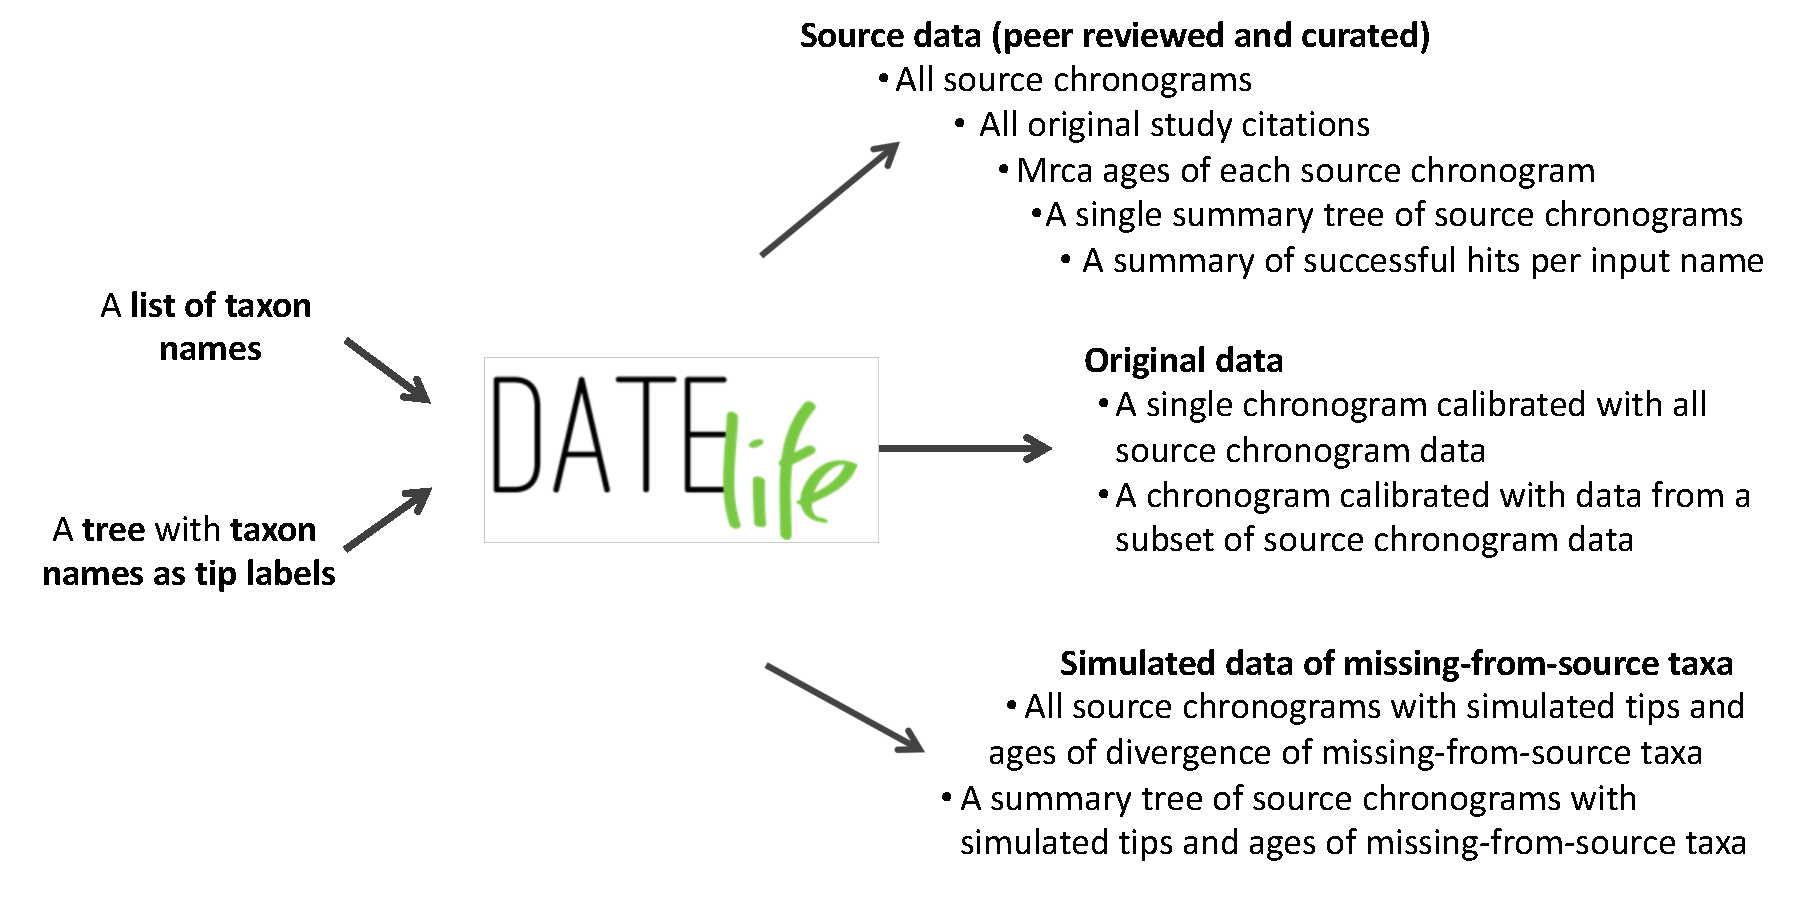
\includegraphics{Fig1.pdf}
\caption{}
\label{fig:workflow}
\end{figure}

\newpage

\begin{figure}[!h]
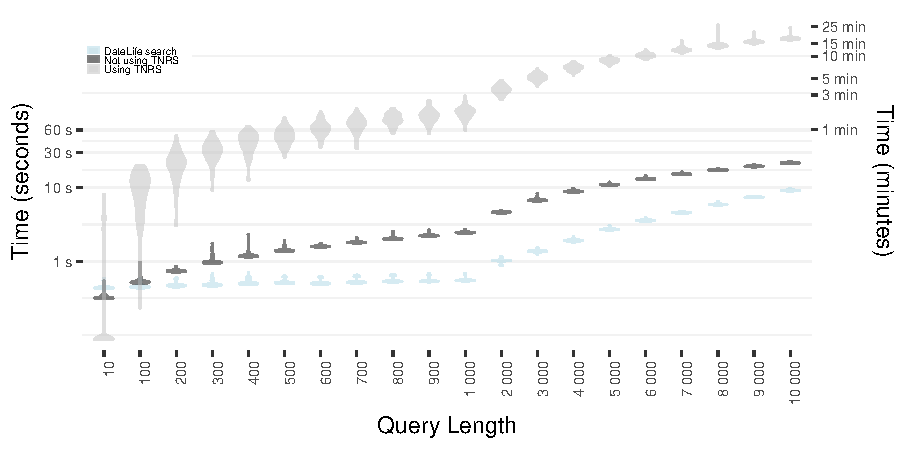
\includegraphics{fig_runtime1.pdf}
\caption{}
\label{fig:runtime1}
\end{figure}

\newpage

\begin{figure}[!h]
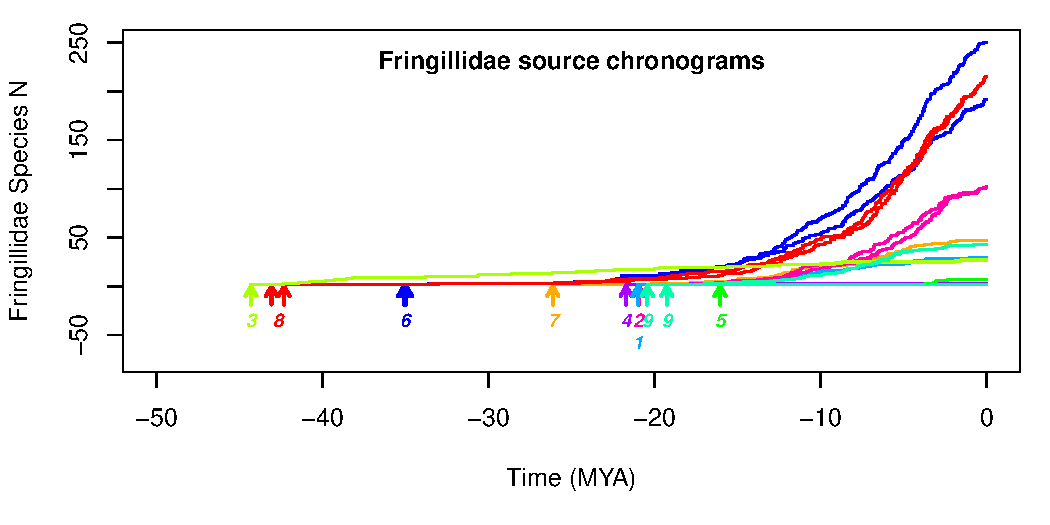
\includegraphics{fig_schronograms1.pdf}
\caption{}
\label{fig:schronograms}
\end{figure}

\newpage

\begin{figure}[!ht]
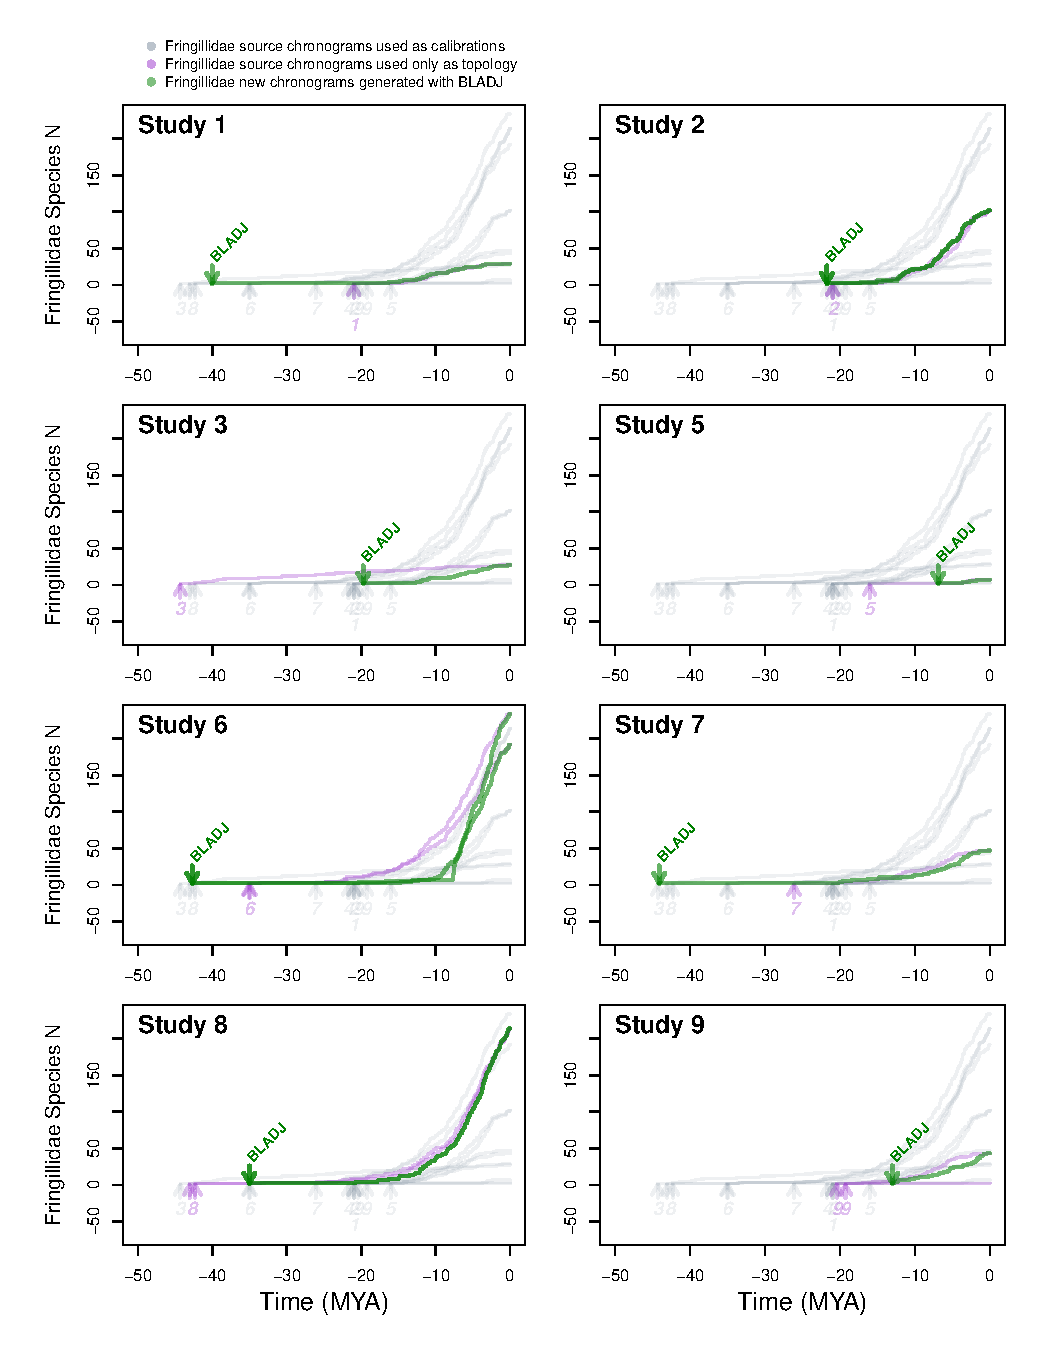
\includegraphics{fig_crossval_bladj.pdf}
\caption{}
\label{fig:cvbladj}
\end{figure}





\newpage
\singlespacing 
\bibliography{../library\_red.bib}

\end{document}